\chapter{Startup Tasks}
\label{sec:tasks} 

In this section, the first steps are described to run the application, create a database or access an existing one, import data and start the management GUI.

\section{Running the Application}

After an \nameref{sec:installation}, simply run the application.

For an AppImage, use e.g.:
\begin{lstlisting}
./ATSDB-release_x86_64.AppImage
\end{lstlisting}

For a self-built application, use e.g.:
\begin{lstlisting}
./build/bin/atsdb_client
\end{lstlisting}

It is recommended to run the application from a console terminal (for issue analysis of the log text), but that is not mandatory.

\section{Configuration Upgrade}

If a previous version of ATSDB has been run on the workstation, the configuration (and additional application data) might be out of date. Since the framework of ATSDB is quite sensitive on being run with the latest configuration an upgrade must be performed. \\


\includegraphics[width=0.5cm]{../../data/icons/hint.png} Please note that this means that the previous configuration will be overwritten, which will unfortunately clear any previous changes made by the user. \\


\includegraphics[width=0.5cm]{../../data/icons/hint.png} Please note that of the previous configuration is older than from v0.5.0 (or newer than the current one), the previous configuration and data folders have to be deleted, clearing any previous changes made by the user. \\


\includegraphics[width=0.5cm]{../../data/icons/hint.png} Please note that with ATSDB version 0.5 (or later) stored configuration data sources can be exported (see \nameref{sec:config_ds_export} and imported again after the upgrade. \\

If an outdated configuration is detected, one of the following dialogs will be shown.

\begin{figure}[H]
    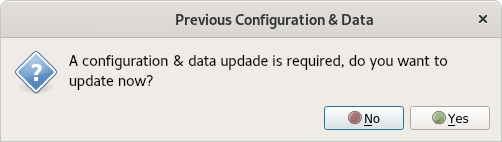
\includegraphics[width=11cm]{../screenshots/config_data_update.png}
  \caption{Configuration and data update}
\end{figure}

\begin{figure}[H]
    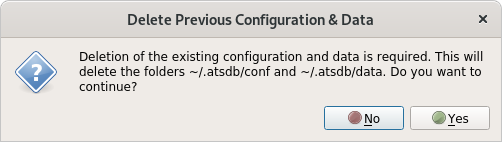
\includegraphics[width=11cm]{../screenshots/config_data_delete_update.png}
  \caption{Configuration and data delete and update}
\end{figure}

If 'Yes' is selected, the update is performed and the application starts. If 'No' is selected, the application will quit. If previous changes to an outdated configuration are of strong importance, please contact the author for support. 

\section{Tasks}

When the application is started the Task window is shown. 

\begin{figure}[H]
  \hspace*{-2.5cm}
    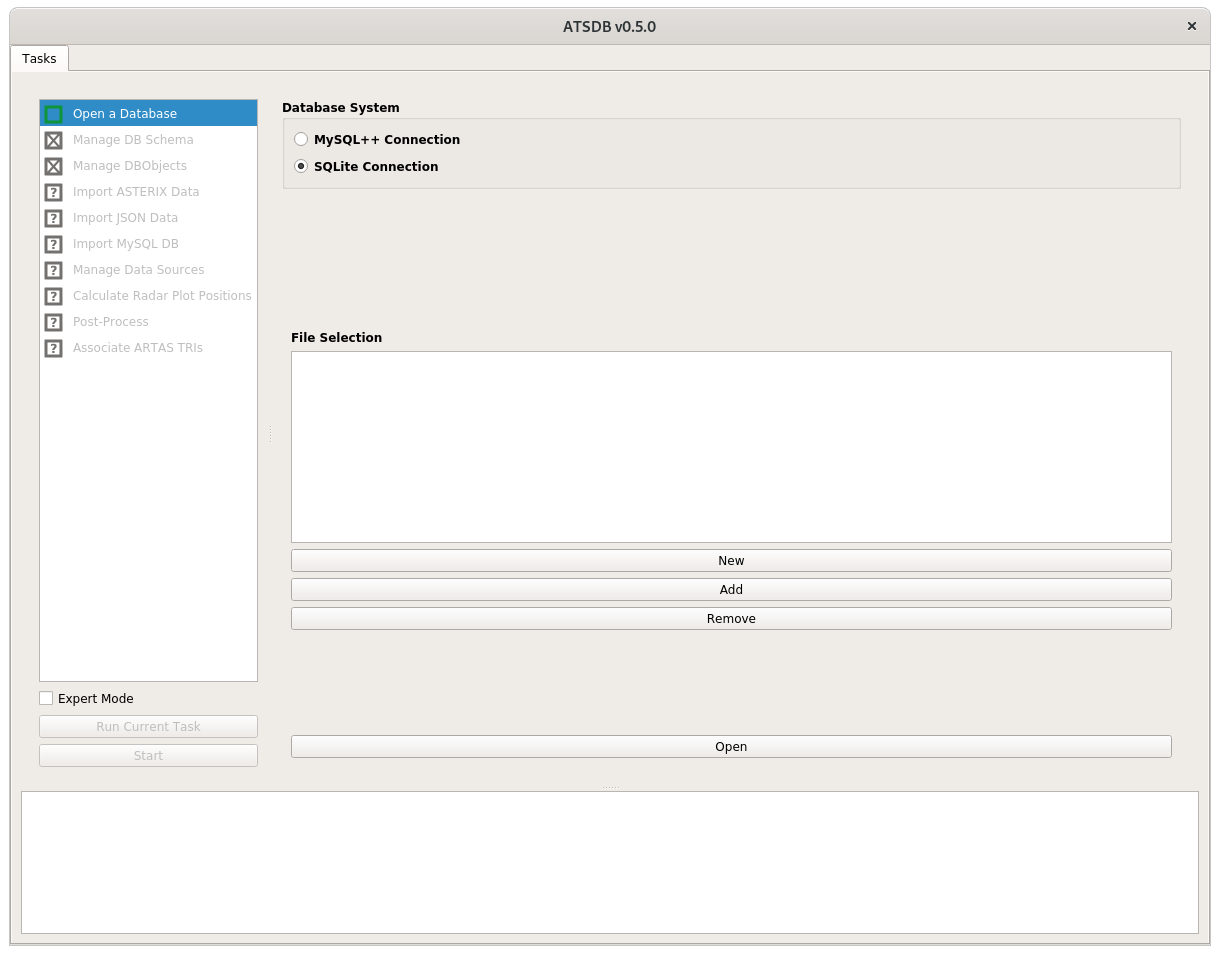
\includegraphics[width=19cm]{../screenshots/task_open_database.png}
  \caption{Startup: Task Window}
\end{figure}

On the left-hand side a number of tasks are listed (task list), on the right hand side a GUI of the currently selected task is shown. On the bottom, a log window is shown. All of these GUI elements can be resized, hidden and shown a again if wanted. \\


The following tasks exist:
\begin{itemize}
 \item Open a Database
 \item Manage DB Schema
 \item Manage DBObjects
 \item Import View Points
 \item Import ASTERIX Data
 \item Import JSON Data
 \item Import MySQL DB
 \item Import GPS Trail
 \item Manage Data Sources
 \item Manage Sectors
 \item Calculate Radar Plot Positions
 \item Post-Process
 \item Associate ARTAS TRIs
\end{itemize}
\  \\

A task (in this context) is an action that has to be performed with interaction of the user. The GUI was designed to guide a user through the workflow of their respective use-case, giving hints about what tasks can and should be performed. \\

If the mouse cursor is hovered over a task, a short tooltip description is given. \\

The following task states are possible:

\begin{itemize}
 \item 
\includegraphics[width=0.5cm]{../../data/icons/todo.png} To Do: Can be run and is recommended
 \item 
\includegraphics[width=0.5cm]{../../data/icons/todo_maybe.png} Not (yet) available
 \item 
\includegraphics[width=0.5cm]{../../data/icons/not_recommended.png} Possible: Can be run but is not recommended
 \item 
\includegraphics[width=0.5cm]{../../data/icons/not_todo.png} Not To Do: Can not be run
 \item 
\includegraphics[width=0.5cm]{../../data/icons/done.png} Done: Already performed
\end{itemize}
\  \\

Tasks which are not available are deactivated (shown in lighter color) and can not be selected. Some tasks are de-activated per default and only become available if the 'Expert Mode' checkbox is checked. For a normal user this is not required.\\

Active tasks can be selected and performed, either by using the 'Run Current Task' button or respective buttons elements in the task's GUI. \\

Whenever a task is done, the state of all other tasks is updated and the next recommended task is selected (if available). The states of the tasks are persisted (at correct application shutdown) in the database, so when re-opening existing ones the task states are shown correctly. \\

Depending on the use-case, some tasks are required, e.g. the Post-Process task. When all required tasks have been performed, the 'Start' button can be used to proceed to the Management window. \\


\includegraphics[width=0.5cm]{../../data/icons/hint.png} Please note that if a previously finalized database is re-opened the 'Start' button is available immediately.

\subfile{task_use_cases}

\subfile{task_open_database}

\subfile{task_manage_schema}
\subfile{task_manage_dbo}

\subfile{task_import_view_points}
\subfile{task_import_asterix}
\subfile{task_import_json}
\subfile{task_import_mysql}
\subfile{task_import_gps}

\subfile{task_manage_datasources}
\subfile{task_manage_sectors}

\subfile{task_calc_radar_pos}

\subfile{task_postprocess}

\subfile{task_associate_artas_tris}

\subfile{task_starting}
